\documentclass{Mayth}
\title{Mayth: 高中数学教学设计}
\author{LeyuDame}
\date{\today}
\begin{document}
\maketitle
\tableofcontents
\chapter{集合与常用逻辑用语}
\section{集合的概念}
\marginnote{2024-7-31}
\subsection{教材分析与教学重难点}
重点: 元素与集合的"属于"关系, 用符号语言刻画集合.

难点: 用描述法表示集合.
\subsection{教学目标}
\begin{enumerate}
	\item 通过示例,了解集合的含义,理解元素与集合的属于关系.
	\item 对于具体问题,能在自然语言和图形语言的基础上,用符号语言表示集合.
	\item 在具体情境中,了解全集与空集的含义.
\end{enumerate}
\subsection{学情分析}

\subsection{教学方法}

\subsection{板书设计}
\begin{boardenv}[集合的概念]
	\begin{enumerate}
		\item 集合的概念\\
		      一般地,我们把研究对象看作是\textbf{元素},把一些元素组成的整体看作是一个\textbf{集合}.
		\item 性质\\
			  确定性、互异性
		\item 属于关系\\
		      $a$属于集合$A$: $a\in A$\\
		      $a$不属于集合$A$: $a\notin A$.
		\item 集合的表示方法\\
		      描述法\\
		      列举法
	\end{enumerate}
\end{boardenv}



\subsection{教学过程}
\begin{intro}[教学片段\cite{HouCongShuXueHaoWanDaoWanHaoShuXueGaoZhongShuXueDiYiKeBuFangCongWan2020}]
	面对新的教师,新的同学,学生往往比较拘谨,不敢表达,这无疑会影响教师教育教学的质量.故而,教师在课程导入时,不妨以集合的“确定性”为背景和学生开一个小玩笑.班长:起立!学生:老师好!教师笑语:同学们好!请所有长头发的同学站一下,其余同学请坐下.(停顿几秒给学生思考)教师继续:(目测包含所有站着的学生)请站着的同学中身高低于2米的坐下.
\end{intro}
\begin{purpose}
	意在建立学生对集合概念的感性认识.“长头发”的不确定性引发学生思考:多长的头发算长头发?部分头发较长的女生不知所措,有的男生也在纠结自己的坐与站的问题.教师快速追加坐下的条件“身高低于2米”,则所有站立的学生坐下,化解了这一部分学生的尴尬.课堂上,师生谈笑间拉近了心理的距离.
\end{purpose}

\begin{intro}
	教师开始本节课的导入语:首先祝贺大家升入高中的学习,老师刚刚以高中数学中“集合”的概念为背景和大家开了一个小玩笑.什么是集合?我们全班的全体同学可以是一个集合,全体的男同学或全体的女同学也都是一个集合,但所有长头发的同学不能构成一个集合,因为集合要满足其内在的个体(元素)是确定的.这也是引发部分同学不确定自己是坐还是站的原因,而站着的同学中“身高低于2米的同学”显然是能够确定的,它是一个集合.集合是现代数学的一个基本概念,也是我们高中数学学习的第一个概念.同学们在后续的学习中要注意数学概念的学习,概念的理解程度决定了我们数学学习的深度,也直接决定了数学解题水平的高低.
\end{intro}
\begin{purpose}
	通过学生不难理解的集合概念,让学生体会数学概念在数学学习中的重要性.教学中,教师不必对集合的概念加以定义,以学生的感性认识理解即可,意在提升学生的学习兴趣和数学认知,也可留下悬念为后续正式学习集合相关知识铺垫情感因素.
\end{purpose}

\subsection{归纳总结与作业布置}
\section{集合的表示方法}
\subsection{教材分析与教学重难点}

\subsection{教学目标}

\subsection{学情分析}

\subsection{板书设计}

\subsection{教学过程}

\subsection{归纳总结与作业布置}

\section{集合的基本运算}
\subsection{教材分析与教学重难点}

\subsection{教学目标}

\subsection{学情分析}

\subsection{板书设计}

\subsection{教学过程}

\subsection{归纳总结与作业布置}

\section{}
\chapter{一元二次函数、方程和不等式}

\chapter{函数的概念与性质}

\chapter{指数函数与对数函数}
\section{指数函数的图象与性质}\marginnote{2024-7-8}
\subsection{教材分析}
《指数函数的图象与性质》选自人教A版必修一函数部分第四章第二节,在此之前,学生已经学过了幂函数的图象与性质,而接下来则是对数函数部分,因此本节内容起着承上启下的作用。
\subsection{学情分析}
学生认知层面,

学生能力层面,
\chapter*{数学建模 建立函数模型解决实际问题}

\chapter{三角函数}


\chapter{平面向量及其应用}
\everymath{\displaystyle}
\newpage
\section{三角形四心的向量表示及应用}

\begin{lemma}[奔驰定理]
    已知点 $O$ 是 $\triangle ABC$ 内部一点. 若 $\mathrm{S}_{\triangle OBC}: \mathrm{S}_{\triangle OAC}: \mathrm{S}_{\triangle OAB}=x: y: z$, 则 $x \lvec{OA} + y \lvec{OB} + z \lvec{OC} = \boldsymbol{0}$;反之亦成立.
    \begin{center}
        \tikzset{every picture/.style={line width=0.75pt}} %set default line width to 0.75pt        
        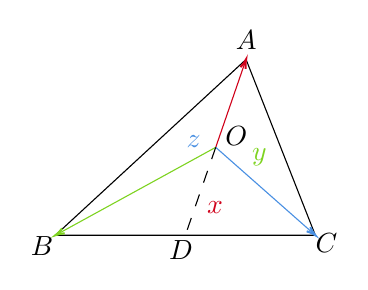
\begin{tikzpicture}[x=0.75pt,y=0.75pt,yscale=-1,xscale=1]
            %uncomment if require: \path (0,300); %set diagram left start at 0, and has height of 300

            %Shape: Triangle [id:dp41718545377725946] 
            \draw   (375.51,83.71) -- (408.89,168.41) -- (283.68,168.41) -- cycle ;
            %Straight Lines [id:da7430270455389383] 
            \draw [color={rgb, 255:red, 208; green, 2; blue, 27 }  ,draw opacity=1 ]   (360.9,126.06) -- (374.86,85.6) ;
            \draw [shift={(375.51,83.71)}, rotate = 109.04] [color={rgb, 255:red, 208; green, 2; blue, 27 }  ,draw opacity=1 ][line width=0.75]    (4.37,-1.32) .. controls (2.78,-0.56) and (1.32,-0.12) .. (0,0) .. controls (1.32,0.12) and (2.78,0.56) .. (4.37,1.32)   ;
            %Straight Lines [id:da21281938084173158] 
            \draw [color={rgb, 255:red, 126; green, 211; blue, 33 }  ,draw opacity=1 ]   (360.9,126.06) -- (285.43,167.45) ;
            \draw [shift={(283.68,168.41)}, rotate = 331.26] [color={rgb, 255:red, 126; green, 211; blue, 33 }  ,draw opacity=1 ][line width=0.75]    (4.37,-1.32) .. controls (2.78,-0.56) and (1.32,-0.12) .. (0,0) .. controls (1.32,0.12) and (2.78,0.56) .. (4.37,1.32)   ;
            %Straight Lines [id:da9898483314704938] 
            \draw [color={rgb, 255:red, 74; green, 144; blue, 226 }  ,draw opacity=1 ]   (360.9,126.06) -- (407.4,167.09) ;
            \draw [shift={(408.89,168.41)}, rotate = 221.42] [color={rgb, 255:red, 74; green, 144; blue, 226 }  ,draw opacity=1 ][line width=0.75]    (4.37,-1.32) .. controls (2.78,-0.56) and (1.32,-0.12) .. (0,0) .. controls (1.32,0.12) and (2.78,0.56) .. (4.37,1.32)   ;
            %Straight Lines [id:da3636995020748923] 
            \draw  [dash pattern={on 4.5pt off 4.5pt}]  (360.9,126.06) -- (346.2,168.61) ;

            % Text Node
            \draw (369.32,68.68) node [anchor=north west][inner sep=0.75pt]    {$A$};
            % Text Node
            \draw (270.57,167.59) node [anchor=north west][inner sep=0.75pt]    {$B$};
            % Text Node
            \draw (407.73,166.45) node [anchor=north west][inner sep=0.75pt]    {$C$};
            % Text Node
            \draw (337.18,169.95) node [anchor=north west][inner sep=0.75pt]    {$D$};
            % Text Node
            \draw (364.32,114.58) node [anchor=north west][inner sep=0.75pt]    {$O$};
            % Text Node
            \draw (355.55,150.73) node [anchor=north west][inner sep=0.75pt]  [color={rgb, 255:red, 208; green, 2; blue, 27 }  ,opacity=1 ]  {$x$};
            % Text Node
            \draw (377.2,125.64) node [anchor=north west][inner sep=0.75pt]  [color={rgb, 255:red, 126; green, 211; blue, 33 }  ,opacity=1 ]  {$y$};
            % Text Node
            \draw (345.63,119.18) node [anchor=north west][inner sep=0.75pt]  [color={rgb, 255:red, 74; green, 144; blue, 226 }  ,opacity=1 ]  {$z$};


        \end{tikzpicture}
    \end{center}
\end{lemma}

\begin{proof}
    延长 $AO$ 交 $BC$ 于点 $D$,

    则$\frac{\mathrm{S}_{\triangle OAB}+\mathrm{S}_{\triangle OAC}}{\mathrm{S}_{\triangle OBC}}=\frac{y+z}{x}=\frac{AO}{OD}$,

    $\therefore x \lvec{OA}=-(y+z) \lvec{OD}$,

    从而$x \lvec{OA}+(y+z) \lvec{OD}=\boldsymbol{0}$. (1)

    又由 $\frac{\mathrm{S}_{\triangle OAB}}{\mathrm{S}_{\triangle OAC}}=\frac{z}{y}=\frac{BD}{CD}$,

    $\therefore y \lvec{BD}=z \lvec{DC}$,

    即 $y(\lvec{OD}-\lvec{OB})=z(\lvec{OC}-\lvec{OD})$,

    $\therefore \lvec{OD}=\frac{y}{y+z} \lvec{OB}+\frac{z}{y+z} \lvec{OC}$,

    代入(1)式得: $x \lvec{OA}+y \lvec{OB}+z \lvec{OC}=\boldsymbol{0}$.
\end{proof}


\subsection{重心的向量表达}
\begin{proposition}
    对于 $\triangle ABC$, 若 $\lvec{GA}+\lvec{GB}+\lvec{GC}=\boldsymbol{0}$, 则 $G$ 是 $\triangle ABC$ 的重心;反之亦成立.
\end{proposition}

\begin{proposition}
    $G$ 是 $\triangle ABC$ 的重心, $P$ 是 $\triangle ABC$ 所在平面上任一点, 则 $\lvec{PG}=\frac{1}{3}(\lvec{PA}+\lvec{PB}+\lvec{PC})$;反之亦成立.
\end{proposition}

\begin{proposition}
    已知 $O$ 是平面上一定点, $A, B, C$ 是平面上不共线的三点, 动点 $P$ 满足 $\lvec{OP}=\lvec{OA}+\lambda(\lvec{AB}+\lvec{AC}), \lambda \in(0,+\infty)$, 则 $P$ 的轨迹一定通过 $\triangle ABC$ 的重心.
\end{proposition}

\subsection{垂心的向量表达}
\begin{proposition}
    对于 $\triangle ABC$, 若 $\tan A \cdot \lvec{HA}+\tan B \cdot \lvec{HB}+\tan C \cdot \lvec{HC}=\boldsymbol{0}$, 则 $H$ 是 $\triangle ABC$ 的垂心;反之亦成立.
\end{proposition}

\begin{proposition}
    $H$ 是 $\triangle ABC$ 所在平面上一点, 若 $\lvec{HA} \cdot \lvec{HB}=\lvec{HB} \cdot \lvec{HC}=\lvec{HC} \cdot \lvec{HA}$, 则 $H$ 是 $\triangle ABC$ 的垂心;反之亦成立.
\end{proposition}

\begin{proposition}
    已知 $O$ 是平面上一定点, $A, B, C$ 是平面上不共线的三点, 动点 $P$ 满足
    $\lvec{OP}=\lvec{OA}+\lambda\left(\frac{\lvec{AB}}{|\lvec{AB}| \cos B}+\frac{\lvec{AC}}{|\lvec{AC}| \cos C}\right), \lambda \in(0,+\infty)$, 则 $P$ 的轨迹一定通过 $\triangle ABC$ 的垂心.
\end{proposition}

\begin{proof}
    由题意得 $\lvec{AP}=\lambda\left(\frac{\lvec{AB}}{|\lvec{AB}| \cos B}+\frac{\lvec{AC}}{|\lvec{AC}| \cos C}\right)$

    \begin{align*}
        \begin{aligned}
             & \text { 而 }\left(\frac{\lvec{AB}}{|\lvec{AB}| \cos B}+\frac{\lvec{AC}}{|\lvec{AC}| \cos C}\right) \cdot \lvec{BC}=\frac{\lvec{AB} \cdot \lvec{BC}}{|\lvec{AB}| \cos B}+\frac{\lvec{AC} \cdot \lvec{BC}}{|\lvec{AC}| \cos C} \\
             & =-|\lvec{BC}|+|\lvec{BC}|                                                                                                                                                                                                   \\
             & =0
        \end{aligned}
    \end{align*}

    $\therefore \lvec{AP} \perp \lvec{BC}$, 动点 $P$ 的轨迹一定通过 $\triangle ABC$ 的垂心.
\end{proof}

\subsection{内心的向量表达}
\begin{proposition}
    对于 $\triangle ABC$, 设 $\mathrm{AB}=c, \mathrm{AC}=b, \mathrm{BC}=a$, 若 $a \cdot \lvec{IA}+b \cdot \lvec{IB}+c \cdot \lvec{IC}=\boldsymbol{0}$, 则点 $I$ 是 $\triangle ABC$ 的内心;反之亦成立.
\end{proposition}

\begin{proof}
    $\because \lvec{IB}=\lvec{IA}+\lvec{AB}, \lvec{IC}=\lvec{IA}+\lvec{AC}$, 代入 $a \cdot \lvec{IA}+b \cdot \lvec{IB}+c \cdot \lvec{IC}=\boldsymbol{0}$ 得\\
    $(a+b+c) \cdot \lvec{IA}+b \cdot \lvec{AB}+c \cdot \lvec{AC}=\boldsymbol{0}$,\\
    $\because b \cdot \lvec{AB}+c \cdot \lvec{AC}=|\lvec{AC}| \cdot \lvec{AB}+|\lvec{AB}| \cdot \lvec{AC}$\\
    $=|\lvec{AB}| \cdot|\lvec{AC}| \cdot\left(\frac{\lvec{AB}}{|\lvec{AB}|}+\frac{\lvec{AC}}{|\lvec{AC}|}\right)$\\
    $=bc\left(\frac{\lvec{AB}}{|\lvec{AB}|}+\frac{\lvec{AC}}{|\lvec{AC}|}\right)$\\
    $\therefore \lvec{AI}=\frac{bc}{a+b+c}\left(\frac{\lvec{AB}}{|\lvec{AB}|}+\frac{\lvec{AC}}{|\lvec{AC}|}\right)$\\
    $\therefore AI$ 与 $\angle BAC$ 的角平分线共线, 即 $AI$ 平分 $\angle BAC$\\
    同理 $BI$ 平分 $\angle ABC, CI$ 平分 $\angle ACB$, 从而 $I$ 是 $\triangle ABC$ 的内心.
\end{proof}

\begin{proposition}
    对于 $\triangle ABC$, 若 $O$ 满足

    $$
        \lvec{OA} \cdot\left(\frac{\lvec{AB}}{|\lvec{AB}|}-\frac{\lvec{AC}}{|\lvec{AC}|}\right)=\lvec{OB} \cdot\left(\frac{\lvec{BA}}{|\lvec{BA}|}-\frac{\lvec{BC}}{|\lvec{BC}|}\right)=\lvec{OC} \cdot\left(\frac{\lvec{CA}}{|\lvec{CA}|}-\frac{\lvec{CB}}{|\lvec{CB}|}\right)=0,
    $$
    则点 $O$ 是 $\triangle ABC$ 的内心;反之亦成立.
\end{proposition}

\subsection{外心的向量表达}
\begin{proposition}
    对于 $\triangle ABC$, 若 $\sin 2A \cdot \lvec{OA}+\sin 2B \cdot \lvec{OB}+\sin 2C \cdot \lvec{OC}=\boldsymbol{0}$, 则 $O$ 是 $\triangle ABC$ 的外心;反之亦成立.
\end{proposition}

\begin{proposition}
    $O$ 是 $\triangle ABC$ 所在平面上一点, 若 $\lvec{OA}^{2}=\lvec{OB}^{2}=\lvec{OC}^{2}$, 则 $O$ 是 $\triangle ABC$ 的外心;反之亦成立.
\end{proposition}

\begin{proposition}
    已知 $O$ 是平面上一定点, $A, B, C$ 是平面上不共线的三点, 动点 $P$ 满足 $\lvec{OP}=\frac{\lvec{OB}+\lvec{OC}}{2}+\lambda\left(\frac{\lvec{AB}}{|\lvec{AB}| \cos B}+\frac{\lvec{AC}}{|\lvec{AC}| \cos C}\right), \lambda \in(0,+\infty)$, 则 $P$ 的轨迹一定通过 $\triangle ABC$ 的外心.
\end{proposition}

\begin{proof}
    设边 $BC$ 的中点为 $M$, 则 $\lvec{OM}=\frac{\lvec{OB}+\lvec{OC}}{2}$, 由题意得
    $$
        \lvec{MP}=\lambda\left(\frac{\lvec{AB}}{|\lvec{AB}| \cos B}+\frac{\lvec{AC}}{|\lvec{AC}| \cos C}\right)
    $$

    \begin{align*}
        \text { 而 }
        \left(\frac{\lvec{AB}}{|\lvec{AB}| \cos B}+\frac{\lvec{AC}}{|\lvec{AC}| \cos C}\right) \cdot \lvec{BC} & =\frac{\lvec{AB} \cdot \lvec{BC}}{|\lvec{AB}| \cos B}+\frac{\lvec{AC} \cdot \lvec{BC}}{|\lvec{AC}| \cos C} \\
                                                                                                               & =-|\lvec{BC}|+|\lvec{BC}|                                                                                  \\
                                                                                                               & =0
    \end{align*}

    $\therefore \lvec{AM} \perp \lvec{BC}, P$ 的轨迹一定通过 $\triangle ABC$ 的外心.
\end{proof}

\subsection{欧拉定理的向量表达}
\begin{proposition}
    若 $O, H$ 分别是 $\triangle ABC$ 的外心和垂心, 则 $\lvec{OH}=\lvec{OA}+\lvec{OB}+\lvec{OC}$.
\end{proposition}

\begin{proof}
    连接 $BO$ 延长交圆 $O$ 于点 $D$, 连接 $AD, CD$, 则 $AD \perp AB, BC \perp CD$\\
    又 $CH \perp AB, AH \perp BC$\\
    $\therefore CH \parallel AD, AH \parallel CD$\\
    $\therefore$ 四边形 $ADCH$ 为平行四边形\\
    $\therefore \lvec{AH}=\lvec{DC}=\lvec{DO}+\lvec{OC}=\lvec{OB}+\lvec{OC}$\\
    $\therefore \lvec{OH}=\lvec{OA}+\lvec{AH}=\lvec{OA}+\lvec{OB}+\lvec{OC}$.
\end{proof}

\tikzset{every picture/.style={line width=0.75pt}} %set default line width to 0.75pt        

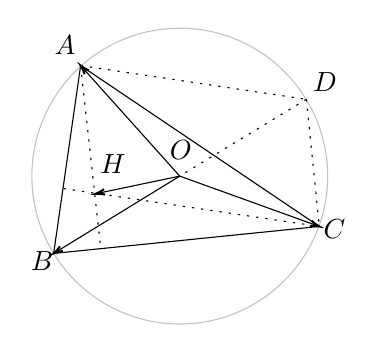
\begin{tikzpicture}[x=0.75pt,y=0.75pt,yscale=-1,xscale=1]
    %uncomment if require: \path (0,300); %set diagram left start at 0, and has height of 300

    %Shape: Circle [id:dp8638038572746185] 
    \draw  [color={rgb, 255:red, 196; green, 193; blue, 193 }  ,draw opacity=1 ] (276.75,155.75) .. controls (276.75,116.4) and (308.65,84.5) .. (348,84.5) .. controls (387.35,84.5) and (419.25,116.4) .. (419.25,155.75) .. controls (419.25,195.1) and (387.35,227) .. (348,227) .. controls (308.65,227) and (276.75,195.1) .. (276.75,155.75) -- cycle ;
    %Straight Lines [id:da5117781865796789] 
    \draw    (300.25,102.5) -- (287.25,193) ;
    %Straight Lines [id:da40133194140523853] 
    \draw    (300.25,102.5) -- (415.25,180) ;
    %Straight Lines [id:da9190277466348651] 
    \draw    (287.25,193) -- (415.25,180) ;
    %Straight Lines [id:da030337826743070506] 
    \draw  [dash pattern={on 0.84pt off 2.51pt}]  (300.25,102.5) -- (310,191.25) ;
    %Straight Lines [id:da6462402259947018] 
    \draw  [dash pattern={on 0.84pt off 2.51pt}]  (292,161.75) -- (415.25,180) ;
    %Straight Lines [id:da6722741273531898] 
    \draw    (348,155.75) -- (288.96,191.95) ;
    \draw [shift={(287.25,193)}, rotate = 328.48] [color={rgb, 255:red, 0; green, 0; blue, 0 }  ][line width=0.75]    (4.37,-1.32) .. controls (2.78,-0.56) and (1.32,-0.12) .. (0,0) .. controls (1.32,0.12) and (2.78,0.56) .. (4.37,1.32)   ;
    %Straight Lines [id:da48269426050329733] 
    \draw    (348,155.75) -- (301.59,103.99) ;
    \draw [shift={(300.25,102.5)}, rotate = 48.12] [color={rgb, 255:red, 0; green, 0; blue, 0 }  ][line width=0.75]    (4.37,-1.32) .. controls (2.78,-0.56) and (1.32,-0.12) .. (0,0) .. controls (1.32,0.12) and (2.78,0.56) .. (4.37,1.32)   ;
    %Straight Lines [id:da4597963546280104] 
    \draw    (348,155.75) -- (413.37,179.32) ;
    \draw [shift={(415.25,180)}, rotate = 199.83] [color={rgb, 255:red, 0; green, 0; blue, 0 }  ][line width=0.75]    (4.37,-1.32) .. controls (2.78,-0.56) and (1.32,-0.12) .. (0,0) .. controls (1.32,0.12) and (2.78,0.56) .. (4.37,1.32)   ;
    %Straight Lines [id:da19024306376007294] 
    \draw [color={rgb, 255:red, 0; green, 0; blue, 0 }  ,draw opacity=1 ]   (348,155.75) -- (309.46,163.84) ;
    \draw [shift={(307.5,164.25)}, rotate = 348.15] [color={rgb, 255:red, 0; green, 0; blue, 0 }  ,draw opacity=1 ][line width=0.75]    (4.37,-1.32) .. controls (2.78,-0.56) and (1.32,-0.12) .. (0,0) .. controls (1.32,0.12) and (2.78,0.56) .. (4.37,1.32)   ;
    %Straight Lines [id:da30127359953371946] 
    \draw  [dash pattern={on 0.84pt off 2.51pt}]  (300.25,102.5) -- (409,118.75) ;
    %Straight Lines [id:da8720800419583445] 
    \draw  [dash pattern={on 0.84pt off 2.51pt}]  (409,118.75) -- (415.25,180) ;
    %Straight Lines [id:da023165060311018726] 
    \draw  [dash pattern={on 0.84pt off 2.51pt}]  (409,118.75) -- (348,155.75) ;

    % Text Node
    \draw (286.5,86.9) node [anchor=north west][inner sep=0.75pt]    {$A$};
    % Text Node
    \draw (275,190.9) node [anchor=north west][inner sep=0.75pt]    {$B$};
    % Text Node
    \draw (416,175.4) node [anchor=north west][inner sep=0.75pt]    {$C$};
    % Text Node
    \draw (411,104.4) node [anchor=north west][inner sep=0.75pt]    {$D$};
    % Text Node
    \draw (342,137.4) node [anchor=north west][inner sep=0.75pt]    {$O$};
    % Text Node
    \draw (308.5,143.9) node [anchor=north west][inner sep=0.75pt]    {$H$};


\end{tikzpicture}
\hspace{2cm}
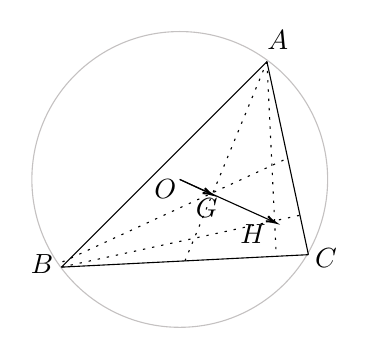
\begin{tikzpicture}[x=0.75pt,y=0.75pt,yscale=-1,xscale=1]
    %uncomment if require: \path (0,300); %set diagram left start at 0, and has height of 300

    %Shape: Circle [id:dp5576661954222375] 
    \draw  [color={rgb, 255:red, 196; green, 193; blue, 193 }  ,draw opacity=1 ] (276.75,155.75) .. controls (276.75,116.4) and (308.65,84.5) .. (348,84.5) .. controls (387.35,84.5) and (419.25,116.4) .. (419.25,155.75) .. controls (419.25,195.1) and (387.35,227) .. (348,227) .. controls (308.65,227) and (276.75,195.1) .. (276.75,155.75) -- cycle ;
    %Straight Lines [id:da7258859971367271] 
    \draw    (390,99) -- (291,198) ;
    %Straight Lines [id:da3156736380760452] 
    \draw    (390,99) -- (410,192) ;
    %Straight Lines [id:da7465470237686334] 
    \draw    (291,198) -- (410,192) ;
    %Straight Lines [id:da033955443365715654] 
    \draw  [dash pattern={on 0.84pt off 2.51pt}]  (291,198) -- (406,173) ;
    %Straight Lines [id:da7312470733297733] 
    \draw  [dash pattern={on 0.84pt off 2.51pt}]  (291.5,195.5) -- (400,145.5) ;
    %Straight Lines [id:da9722534008421468] 
    \draw    (348,155.75) -- (361.69,162.15) ;
    \draw [shift={(363.5,163)}, rotate = 205.07] [color={rgb, 255:red, 0; green, 0; blue, 0 }  ][line width=0.75]    (4.37,-1.32) .. controls (2.78,-0.56) and (1.32,-0.12) .. (0,0) .. controls (1.32,0.12) and (2.78,0.56) .. (4.37,1.32)   ;
    %Straight Lines [id:da5490453987009081] 
    \draw    (348,155.75) -- (392.18,175.68) ;
    \draw [shift={(394,176.5)}, rotate = 204.28] [color={rgb, 255:red, 0; green, 0; blue, 0 }  ][line width=0.75]    (4.37,-1.32) .. controls (2.78,-0.56) and (1.32,-0.12) .. (0,0) .. controls (1.32,0.12) and (2.78,0.56) .. (4.37,1.32)   ;
    %Straight Lines [id:da9976698491167126] 
    \draw  [dash pattern={on 0.84pt off 2.51pt}]  (390,99) -- (394.5,192.5) ;
    %Straight Lines [id:da4368693118593838] 
    \draw  [dash pattern={on 0.84pt off 2.51pt}]  (350.5,195) -- (390,99) ;

    % Text Node
    \draw (389,82.9) node [anchor=north west][inner sep=0.75pt]    {$A$};
    % Text Node
    \draw (275,190.9) node [anchor=north west][inner sep=0.75pt]    {$B$};
    % Text Node
    \draw (412,187.9) node [anchor=north west][inner sep=0.75pt]    {$C$};
    % Text Node
    \draw (354.5,163.9) node [anchor=north west][inner sep=0.75pt]    {$G$};
    % Text Node
    \draw (334.5,154.4) node [anchor=north west][inner sep=0.75pt]    {$O$};
    % Text Node
    \draw (376,176.4) node [anchor=north west][inner sep=0.75pt]    {$H$};


\end{tikzpicture}

\begin{proposition}
    若 $O, G, H$ 分别是 $\triangle ABC$ 的外心, 重心, 垂心, 则 $\lvec{OG}=\frac{1}{3} \lvec{OH}$.
\end{proposition}

\begin{proof}
    $\because G$ 是重心, 由命题 2 知 $\lvec{OG}=\frac{1}{3}(\lvec{OA}+\lvec{OB}+\lvec{OC})$\\
    又由命题 12 知 $\lvec{OH}=\lvec{OA}+\lvec{OB}+\lvec{OC}$\\
    $\therefore \lvec{OG}=\frac{1}{3} \lvec{OH}$.
\end{proof}

\section{练习题}
\begin{exercise}
    已知 $O$ 是 $\triangle ABC$ 的重心, 点 $P$ 满足 $\lvec{OP}=\frac{1}{3}\left(\frac{1}{2} \lvec{OA}+\frac{1}{2} \lvec{OB}+2 \lvec{OC}\right)$, 则点 $P$ 一定是 $\triangle ABC$ 的( \quad ). \\
    A. $AB$ 边中线的中点 \qquad B. $AB$ 边中线的三等分点(非重心) \\
    C. 重心 \qquad D. $AB$ 边的中点
\end{exercise}

\begin{exercise}
    $O$ 是 $\triangle ABC$ 所在平面上一点, 若 $\lvec{OA}^{2}+\lvec{BC}^{2}=\lvec{OB}^{2}+\lvec{CA}^{2}=\lvec{OC}^{2}+\lvec{AB}^{2}$, 则 $O$ 是 $\triangle ABC$ 的( \quad ). \\
    A. 外心 \qquad B. 内心 \qquad C. 垂心 \qquad D. 重心
\end{exercise}

\begin{exercise}
    $P$ 是 $\triangle ABC$ 所在平面上一点, 若 $\lvec{PA} \cdot \lvec{PB}+\lvec{PB} \cdot \lvec{PC}+\lvec{PA} \cdot \lvec{PC}=0$, 则 $P$ 是 $\triangle ABC$ 的( \quad ). \\
    A. 外心 \qquad B. 内心 \qquad C. 垂心 \qquad D. 重心
\end{exercise}

\begin{exercise}
    $P$ 是 $\triangle ABC$ 所在平面上一点, 若 $\lvec{CA}^{2}=\lvec{CB}^{2}-2 \lvec{AB} \cdot \lvec{CP}$, 则 $P$ 的轨迹一定通过 $\triangle ABC$ 的( \quad ). \\
    A. 外心 \qquad B. 内心 \qquad C. 垂心 \qquad D. 重心
\end{exercise}

\begin{exercise}
    已知非零向量 $\lvec{AB}, ~ \lvec{AC}$ 满足 $\left(\frac{\lvec{AB}}{|\lvec{AB}|}+\frac{\lvec{AC}}{|\lvec{AC}|}\right) \cdot \lvec{BC}=0$, 且 $\frac{\lvec{AB}}{|\lvec{AB}|} \cdot \frac{\lvec{AC}}{|\lvec{AC}|}=\frac{1}{2}$, 则 $\triangle ABC$ 为( \quad ). \\
    A. 三边均不相等的三角 \qquad B. 直角三角形 \\
    C. 等腰非等边三角形 \qquad D. 等边三角形
\end{exercise}

\begin{exercise}
    $P$ 是 $\triangle ABC$ 所在平面内与 $A$ 不重合的一点, 且满足 $\lvec{AB}+\lvec{AC}=3 \lvec{AP}$, 则 $P$ 是 $\triangle ABC$ 的( \quad ). \\
    A. 外心 \qquad B. 内心 \qquad C. 垂心 \qquad D. 重心
\end{exercise}

\begin{exercise}
    已知 $O$ 是 $\triangle ABC$ 的外接圆的圆心, 半径为 1, 且 $\lvec{OA}+\lvec{OB}+\lvec{OC}=\boldsymbol{0}$, 则 $\lvec{OA} \cdot \lvec{OB}$ 等于 ( \quad ).
\end{exercise}

\begin{exercise}
    $\triangle ABC$ 的外接圆圆心为 $O$, 两条边上的高的交点为 $H$, 若 $\lvec{OH}=m(\lvec{OA}+\lvec{OB}+\lvec{OC})$, 则实数 $m=$ ( \quad ).
\end{exercise}

\begin{exercise}
    已知 $G$ 是 $\triangle ABC$ 的重心, 过 $G$ 作直线与 $AB, AC$ 分别相交于 $M, N$ 两点, 若 $\lvec{AM}=x \lvec{AB}, \lvec{AN}=y \lvec{AC}$, 则 $\frac{1}{x}+\frac{1}{y}=$ ( \quad ).
\end{exercise}

\texttt{答案: 1-6 BCCADD \quad 7. -1/2 \quad  8. 1  \quad 9. 3}
\chapter{复数}

\chapter{立体几何初步}
%\section{基本立体图形}
%\section{立体图形的直观图I}
%\section{立体图形的直观图II}
%\section{棱柱、棱锥、棱台的表面积与体积}
%\section{圆柱、圆锥、圆台的表面积与体积}
\section{球的表面积与体积}
\marginnote{2024-4-29}
\subsection{球的表面积}
我们在初中都学过圆的面积, 设圆的半径为 $r$, 则圆的面积为
 $$
 S = \uppi r^{2}. 
 $$ 
 上式说明圆的面积和半径有关, 进一步地讲, 圆的面积作为二维平面上的度量, 它和圆的半径的平方成正比. 此外, 圆的面积还包含了常数 $\uppi$. 类似地, 同样是求面积, 我们是否可以推测球的表面积也和球的半径平方成正比呢?是否也和常数 $\uppi$ 有关呢?
\begin{formula}[球的表面积]
	设球的半径为 $r$, 则球的表面积
	$$
		S_{\text{球}}= 4 \uppi r^{2}.
	$$
\end{formula}
下面给出一个不太严谨的球的表面积公式的证明方法, 主要是利用圆柱侧面积来近似代替球的表面积. 
\begin{proof}
  把一个半径为 $r$ 的球的上半球横向切成 $n$ (无穷大)份, 每份等高并且把每份看成一个类似圆柱, 其中半径等于底面圆半径, 则从下到上第 $k$ 个圆柱的侧面积为
  $$
  S(k)=2 \uppi r_k h .
  $$
  $$
  \begin{aligned}
  & \because h=\frac{r}{n}, r_k=\sqrt{r^2-(k h)^2}, \\
  & \therefore S(k)=\frac{2 \uppi r}{n} \sqrt{r^2-(k h)^2}=2 \uppi r^2 \sqrt{\frac{1}{n^2}-\frac{k^2}{n^4}} . \\
  & \therefore S_{\text {球 }}=\lim _{n \rightarrow+\infty} 2[S(1)+S(2)+\cdots+S(n)]=4 \uppi r^2 .
  \end{aligned}
  $$
\end{proof}  

\begin{formula}[球的体积]
	设球的半径为 $r$, 则球的体积
  $$
  V_{\text{球}}=\frac{4}{3} \uppi r^{3}.
  $$
\end{formula}

\begin{example}
	如图 8.3-4, 某种浮标由两个半球和一个圆柱黏合而成,半球的直径是 $0.3 \mathrm{~m}$, 圆柱高 $0.6 \mathrm{~m}$. 如果在浮标表面涂一层防水漆, 每平方米需要 $0.5 \mathrm{~kg}$ 涂料, 那么给 1000 个这样的浮标涂防水漆需要多少涂料? ( $\uppi$ 取 3.14)
\end{example}
\begin{solution}
一个浮标的表面积为
	$$
		2 \uppi \times 0.15 \times 0.6+4 \uppi \times 0.15^2=0.8478\left(\mathrm{~m}^2\right),
	$$

	所以给 1000 个这样的浮标涂防水漆约需涂料
	$$
		0.8478 \times 0.5 \times 1000=423.9(\mathrm{~kg}) .
	$$
\end{solution}


类比利用圆周长求圆面积的方法, 我们可以利用球的表面积求球的体积. 如图8.3-5,把球 $O$ 的表面分成 $n$ 个小网格, 连接球心 $O$ 和每个小网格的顶点, 整个球体就被分割成 $n$ 个 “小锥体”.

当 $n$ 越大, 每个小网格越小时, 每个 “小锥体” 的底面就越平, “小锥体” 就越近似于棱雉, 其高越近似于球半径 $R$. 设 $O-A B C D$ 是其中一个 “小锥体”, 它的体积
$$
V_{O-A B C D} \approx \frac{1}{3} S_{A B C D} R . 
$$

由于球的体积就是这 $n$ 个 “小锥体” 的体积之和, 而这 $n$ 个 “小锥体” 的底面积之和就是球的表面积. 因此, 球的体积
$$
V_{\text {球 }}=\frac{1}{3} S_{\text {球 }} R=\frac{1}{3} \times 4 \uppi R^2 \cdot R=\frac{4}{3} \uppi R^3 . 
$$

由此, 我们得到球的体积公式
$$
V_{\text {球 }}=\frac{4}{3} \uppi R^3 .
$$
\end{document}